% 2016 年全国卷Ⅱ理科第 19 题：菱形底面与折起后的 D'
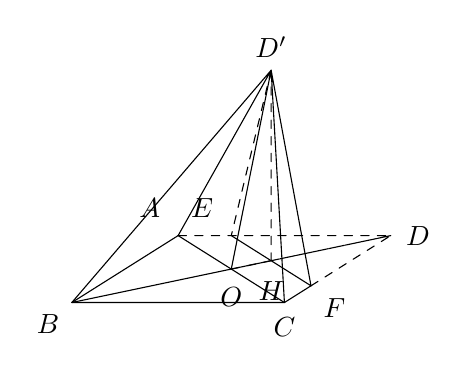
\begin{tikzpicture}[line cap=round,line join=round]
  \coordinate (A)  at (0,1.1);
  \coordinate (B)  at (-1.35,0.25);
  \coordinate (C)  at (1.35,0.25);
  \coordinate (D)  at (2.7,1.1);
  \coordinate (O)  at (0.675,0.675);
  \coordinate (E)  at (0.675,1.1);
  \coordinate (F)  at (1.6875,0.4625);
  \coordinate (H)  at (1.18125,0.78125);
  \coordinate (Dp) at (1.18125,3.2);

  % 按原图保留虚线段，不另作线型含义解释
  \draw[dashed] (A)--(D) (F)--(D) (H)--(D) (Dp)--(H) (Dp)--(E) (O)--(D);

  % 菱形、对角线、折痕与折起后的连线
  \draw (A)--(B)--(C);
  \draw (A)--(C);
  \draw (B)--(H);
  \draw (E)--(F);
  \draw (C)--(F);
  \draw (Dp)--(A) (Dp)--(B) (Dp)--(C) (Dp)--(F) (Dp)--(O);

  \node[above left=3pt] at (A) {$A$};
  \node[below left=1pt] at (B) {$B$};
  \node[below=2pt] at (C) {$C$};
  \node[right=2pt] at (D) {$D$};
  \node[above left=3pt] at (E) {$E$};
  \node[below right=1pt] at (F) {$F$};
  \node[below=3pt] at (O) {$O$};
  \node[below=4pt] at (H) {$H$};
  \node[above=1pt] at (Dp) {$D'$};
\end{tikzpicture}
